\subsection{Constraint Solving}
\label{sec:constraint-solving}

% TODO: Check out 132, 133, 134 of the overview

Another approach to program synthesis is to reduce the problem to that of
constraint solving by the use of off-the-shelf automated constraint
solvers~\cite{Shi:2019:FCS,Feng:2018:PSU,Feng:2017:CST,Feng:2017:CSC,Solar-Lezama:2008,Jha:oracle:2010}
(typically SAT or SMT solvers).

% TODO: Propositional formulas, SAT, SMT, LIA and simple encoding examples --> preliminaries

One idea is to encode the specification in a logical constraint whose solution
corresponds to the desired program. \citeauthor{Gulwani2017} illustrate this
idea nicely with an example~\cite{Gulwani2017} which we adapt here.
Suppose our programs are composed of operations over two input bitvectors, $x$
and $y$ of length eight:

% FIXME
\begin{figure}[h!]
  \centering
  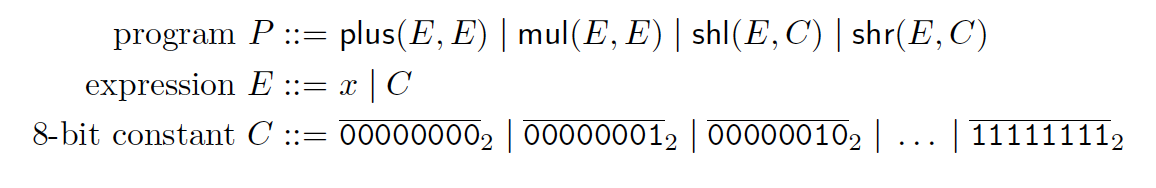
\includegraphics[width=\textwidth]{assets/constraint-solving-example.png}
  \caption{FIXME: This example is a placeholder and should be adapted.}
\end{figure}

We consider an expression to be the input variable $x$ or an 8-bit constant. A
program consists of additions and multiplications between expressions, or of
shift left/right operations over an expression by a constant.

Imagine we are interested in a program that \todo{<insert interesting bit
  twiddling hack>}{check Hacker's Delight}. In the theory of
\todo{bitvectors}{missing ref}, the program we are interested in can be encoded
by the formula \todo{<insert formula here>}{add formula correspondent to the
hack}. To find the program we can write the constraints in the SMT-LIB format
and feed them to an SMT solver:

% FIXME
\begin{figure}[h!]
  \centering
  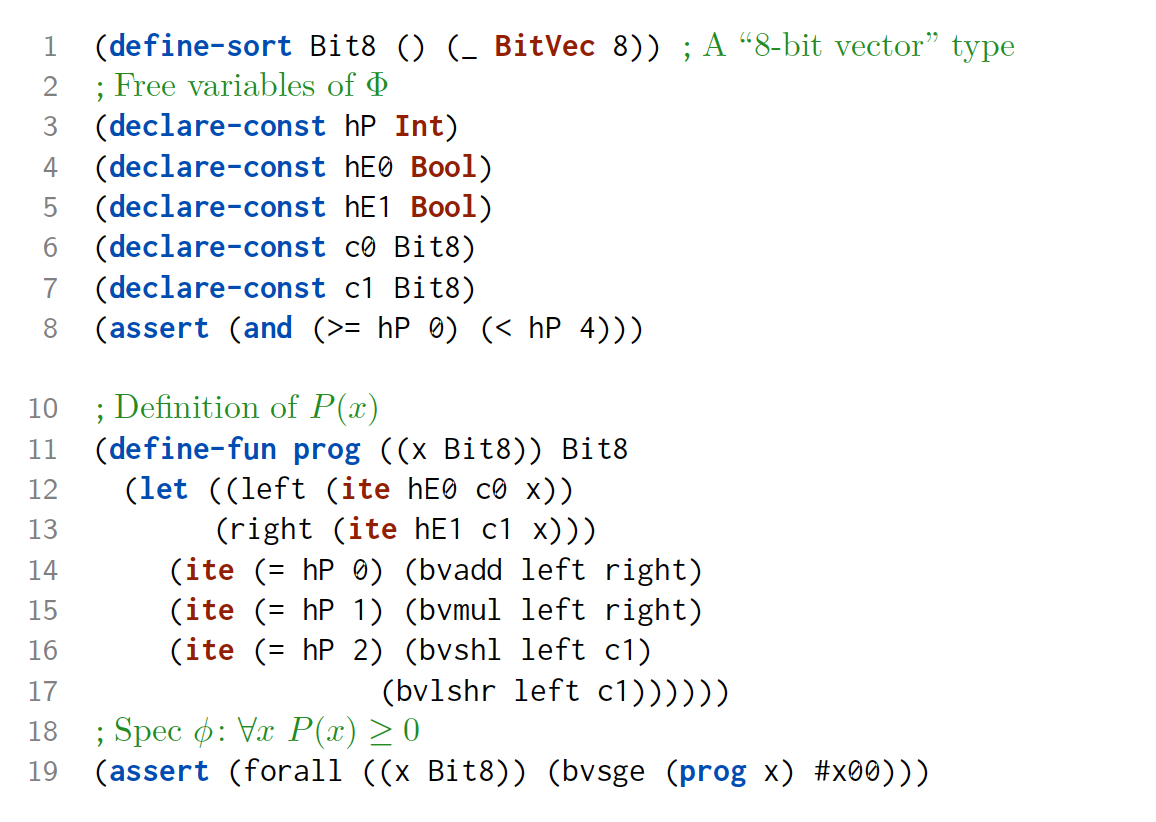
\includegraphics[width=\textwidth]{assets/constraint-solving-smtlib.png}
  \caption{FIXME: This example is a placeholder and should be adapted.}
\end{figure}

This example shows an end-to-end constraint solving approach to program
synthesis. However, enconding the problem this way can sometimes be non-trivial
or time-consuming. This idea led to the appearance of the concept of
\textit{solver-aided programming}, where programming languages are enlarged with
high-level constructs that give the user access to synthesis without having to
deal with the constraint solvers directly.

For example, \citeauthor{Gulwani2017} describe the SKETCH system as a ``compiler
[that] relies on a SAT solver to materialize some language constructs''.
ROSETTE~\cite{Torlak:2013:GSL} is a framework for developing solver-aided
programming languages embedded in Racket that provides constructs not only for
synthesis, but also for verification, debugging and angelic execution.
% SMTEN?
% Metasketching, symbolic profiling?

\subsubsection{Component-Based Synthesis}
\label{sec:components}

% TODO Check
% 12, 13, 22, 34 of Gulwani2017
% 9, 16, 17 of Feng:2017:CSC

One area of program synthesis where constraint solving techniques have seen
considerable use is that of \textit{component-based
synthesis}~\cite{Shi:2019:FCS,Feng:2018:PSU,Feng:2017:CST,Feng:2017:CSC,Jha:oracle:2010}.
In component-based synthesis we are interested in finding a loop-free program
made out of a combination of fundamental building blocks called
\textit{components}. These components could be, for example, methods in a
library \gls{api}~\cite{Shi:2019:FCS,Feng:2017:CSC}, and they form the syntactic
bias for the programs we want to find. They may also be supplemented by
additional constraints in the form of logical formulas~\cite{Feng:2018:PSU}.

% TODO Examples: SyPet and FrAngel
% Also, FrAngel adds control structures to the problem

% TODO
% - Conflict-driven, distinguishing inputs
% - Inductive Logic Programming

